\chapter{Enumeration of Unlabeled Rooted Trees}\label{chapter:rootred_tree_enum}

This Chapter describes the verification of an algorithm enumerating all unlabeled rooted trees with a specific number of nodes.
Let $G = (V,E,r)$ denote the rooted graph with vertex set $V$, edge set $E$ and a distinguished root $r \in V$.

\begin{isabellebox}
\isacommand{locale}\isamarkupfalse%
\ rgraph\ {\isacharequal}{\kern0pt}\ graph{\isacharunderscore}{\kern0pt}system\ {\isacharplus}{\kern0pt}\isanewline
\ \ \isakeyword{fixes}\ r\isanewline
\ \ \isakeyword{assumes}\ root{\isacharunderscore}{\kern0pt}wf{\isacharcolon}{\kern0pt}\ {\isachardoublequoteopen}r\ {\isasymin}\ V{\isachardoublequoteclose}
\end{isabellebox}

Similarly, a rooted tree is a tree with a fixed root.

\begin{isabellebox}
    \isacommand{locale}\isamarkupfalse%
    \ rtree\ {\isacharequal}{\kern0pt}\ tree\ {\isacharplus}{\kern0pt}\ rgraph
\end{isabellebox}

As can be seen in the definition the nodes of rooted graphs are still labeled.
To get a notion of unlabeled trees we define isomorphism on these graphs.
A graph isomorphism for (unrooted) graphs is a bijection between the vertex sets of two graphs which preserves edge connectivity.

\begin{isabellebox}
\isacommand{locale}\isamarkupfalse%
\ graph{\isacharunderscore}{\kern0pt}isomorphism\ {\isacharequal}{\kern0pt}\isanewline
\ \ G{\isacharcolon}{\kern0pt}\ graph{\isacharunderscore}{\kern0pt}system\ V\isactrlsub G\ E\isactrlsub G\ \isakeyword{for}\ V\isactrlsub G\ E\isactrlsub G\ {\isacharplus}{\kern0pt}\isanewline
\ \ \isakeyword{fixes}\ V\isactrlsub H\ E\isactrlsub H\ f\isanewline
\ \ \isakeyword{assumes}\ bij{\isacharunderscore}{\kern0pt}f{\isacharcolon}{\kern0pt}\ {\isachardoublequoteopen}bij{\isacharunderscore}{\kern0pt}betw\ f\ V\isactrlsub G\ V\isactrlsub H{\isachardoublequoteclose}\isanewline
\ \ \isakeyword{and}\ edge{\isacharunderscore}{\kern0pt}preserving{\isacharcolon}{\kern0pt}\ {\isachardoublequoteopen}{\isacharparenleft}{\kern0pt}{\isacharparenleft}{\kern0pt}{\isacharbackquote}{\kern0pt}{\isacharparenright}{\kern0pt}\ f{\isacharparenright}{\kern0pt}\ {\isacharbackquote}{\kern0pt}\ E\isactrlsub G\ {\isacharequal}{\kern0pt}\ E\isactrlsub H{\isachardoublequoteclose}
\end{isabellebox}

Similarly, graph isomorphism is defined on rooted graphs with the additional requirement that the isomorphism also preserves the root node.

\begin{isabellebox}
    \isacommand{locale}\isamarkupfalse%
    \ rgraph{\isacharunderscore}{\kern0pt}isomorphism\ {\isacharequal}{\kern0pt}\isanewline
    \ \ G{\isacharcolon}{\kern0pt}\ rgraph\ V\isactrlsub G\ E\isactrlsub G\ r\isactrlsub G\ {\isacharplus}{\kern0pt}\ graph{\isacharunderscore}{\kern0pt}isomorphism\ V\isactrlsub G\ E\isactrlsub G\ V\isactrlsub H\ E\isactrlsub H\ f\ \isakeyword{for}\ V\isactrlsub G\ E\isactrlsub G\ r\isactrlsub G\ V\isactrlsub H\ E\isactrlsub H\ r\isactrlsub H\ f\ {\isacharplus}{\kern0pt}\isanewline
    \ \ \isakeyword{assumes}\ root{\isacharunderscore}{\kern0pt}preserving{\isacharcolon}{\kern0pt}\ {\isachardoublequoteopen}f\ r\isactrlsub G\ {\isacharequal}{\kern0pt}\ r\isactrlsub H{\isachardoublequoteclose}
\end{isabellebox}

The algorithm described here produces a list of all rooted trees with n vertices modulo isomorphism.
That is, every rooted tree is isomorphic to exactly one rooted tree in the resulting list.


\section{Algorithm}

The idea of the algorithm is based on one described by Beyer and Hedetniemi \parencite{beyer}.
It works on ordered, rooted trees.
An ordered, rooted tree is a rooted tree with a linear order with which subtrees can be ordered.
We will represent such a tree graphically as in Figure \ref{fig:example_rooted_trees} by drawing the root node at the top and the subtrees in the corresponding order beneath it.
Since we are interested in unlabeled trees, node labels will generally be omitted.
The two trees shown differ in the ordering of their subtrees but represent the same underlying rooted tree.
Of the possibly many ordered trees corresponding to a rooted tree, one canonical tree will be defined.
For this, a linear order will be defined on ordered rooted trees.
First we define the type of ordered rooted trees as the root node with a list of ordered subtrees.

\begin{isabellebox}
\isacommand{datatype}\isamarkupfalse%
\ tree\ {\isacharequal}{\kern0pt}\ Node\ {\isachardoublequoteopen}tree\ list{\isachardoublequoteclose}
\end{isabellebox}

This order defined on these trees will be the reversed lexicographical ordering.
No tree is smaller than the singleton tree (a tree only containing a root node).
The singleton tree is smaller than every other tree besides itself.
Otherwise, the subtrees are compared element wise from the back.
To simplify the definition in a functional setting, we first define the regular lexicographical order on trees and then define the desired ordering by mirroring its arguments.

\begin{figure}[htpb]
    \centering
    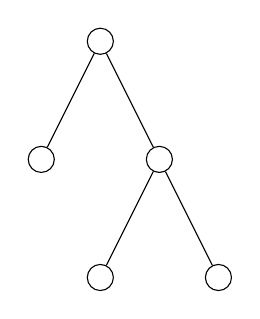
\begin{tikzpicture}
    \tikzstyle{every node}=[circle, draw]
    \node[circle, draw] {}
        child {node {}}
        child {node {}
            child {node {}}
            child {node {}}
    };
    \end{tikzpicture}
    \hspace{2cm}
    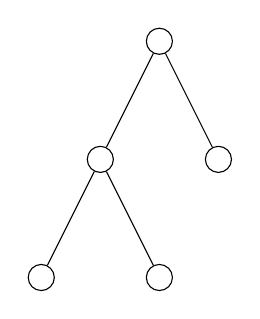
\begin{tikzpicture}
        \tikzstyle{every node}=[circle, draw]
        \node[circle, draw] {}
            child {node {}
                child {node {}}
                child {node {}}}
            child {node {}};
\end{tikzpicture}
\caption{Example rooted trees}
\label{fig:example_rooted_trees}
\end{figure}

\begin{isabellebox}
    \isacommand{fun}\isamarkupfalse%
    \ lexord{\isacharunderscore}{\kern0pt}tree\ \isakeyword{where}\isanewline
    \ \ {\isachardoublequoteopen}lexord{\isacharunderscore}{\kern0pt}tree\ t\ {\isacharparenleft}{\kern0pt}Node\ {\isacharbrackleft}{\kern0pt}{\isacharbrackright}{\kern0pt}{\isacharparenright}{\kern0pt}\ {\isasymlongleftrightarrow}\ False{\isachardoublequoteclose}\isanewline
    {\isacharbar}{\kern0pt}\ {\isachardoublequoteopen}lexord{\isacharunderscore}{\kern0pt}tree\ {\isacharparenleft}{\kern0pt}Node\ {\isacharbrackleft}{\kern0pt}{\isacharbrackright}{\kern0pt}{\isacharparenright}{\kern0pt}\ r\ {\isasymlongleftrightarrow}\ True{\isachardoublequoteclose}\isanewline
    {\isacharbar}{\kern0pt}\ {\isachardoublequoteopen}lexord{\isacharunderscore}{\kern0pt}tree\ {\isacharparenleft}{\kern0pt}Node\ {\isacharparenleft}{\kern0pt}t{\isacharhash}{\kern0pt}ts{\isacharparenright}{\kern0pt}{\isacharparenright}{\kern0pt}\ {\isacharparenleft}{\kern0pt}Node\ {\isacharparenleft}{\kern0pt}r{\isacharhash}{\kern0pt}rs{\isacharparenright}{\kern0pt}{\isacharparenright}{\kern0pt}\ {\isasymlongleftrightarrow}\isanewline
    \ \ \ \ lexord{\isacharunderscore}{\kern0pt}tree\ t\ r\ {\isasymor}\ {\isacharparenleft}{\kern0pt}t\ {\isacharequal}{\kern0pt}\ r\ {\isasymand}\ lexord{\isacharunderscore}{\kern0pt}tree\ {\isacharparenleft}{\kern0pt}Node\ ts{\isacharparenright}{\kern0pt}\ {\isacharparenleft}{\kern0pt}Node\ rs{\isacharparenright}{\kern0pt}{\isacharparenright}{\kern0pt}{\isachardoublequoteclose}\isanewline
    \isanewline
    \isacommand{fun}\isamarkupfalse%
    \ mirror\ {\isacharcolon}{\kern0pt}{\isacharcolon}{\kern0pt}\ {\isachardoublequoteopen}tree\ {\isasymRightarrow}\ tree{\isachardoublequoteclose}\ \isakeyword{where}\isanewline
    \ \ {\isachardoublequoteopen}mirror\ {\isacharparenleft}{\kern0pt}Node\ ts{\isacharparenright}{\kern0pt}\ {\isacharequal}{\kern0pt}\ Node\ {\isacharparenleft}{\kern0pt}map\ mirror\ {\isacharparenleft}{\kern0pt}rev\ ts{\isacharparenright}{\kern0pt}{\isacharparenright}{\kern0pt}{\isachardoublequoteclose}\isanewline
    \isanewline
    \isacommand{definition}\isamarkupfalse%
    \isanewline
    \ \ tree{\isacharunderscore}{\kern0pt}less{\isacharunderscore}{\kern0pt}def{\isacharcolon}{\kern0pt}\ {\isachardoublequoteopen}{\isacharparenleft}{\kern0pt}t{\isacharcolon}{\kern0pt}{\isacharcolon}{\kern0pt}tree{\isacharparenright}{\kern0pt}\ {\isacharless}{\kern0pt}\ r\ {\isasymlongleftrightarrow}\ lexord{\isacharunderscore}{\kern0pt}tree\ {\isacharparenleft}{\kern0pt}mirror\ t{\isacharparenright}{\kern0pt}\ {\isacharparenleft}{\kern0pt}mirror\ r{\isacharparenright}{\kern0pt}{\isachardoublequoteclose}
\end{isabellebox}

For a rooted tree $T$, we now define the canonical ordered tree as the greatest ordered tree corresponding to $T$.
In Figure \ref{fig:example_rooted_trees} the left tree is the canonical ordered tree.

The algorithm will produce all canonical ordered trees.
Instead of working with rooted trees directly, the algorithm of Beyer and Hedetniemi uses an alternative representation of rooted trees, namely level sequences.
The algorithm described here enumerates rooted trees in the same order but is defined recursively on a recursive tree datatype instead of on the level sequences.

To traverse all rooted trees a successor function is defined giving the next smallest canonical tree.
To accomplish this, some auxiliary functions are needed.
We define a function that trims a tree, $trim\_tree\ n\ t$ trims t to n nodes by removing nodes in postorder until the tree has at most n nodes.
See Figure \ref{fig:trim_tree_example} for an example of how $trim\_tree$ works.

\begin{figure}[htpb]
\centering
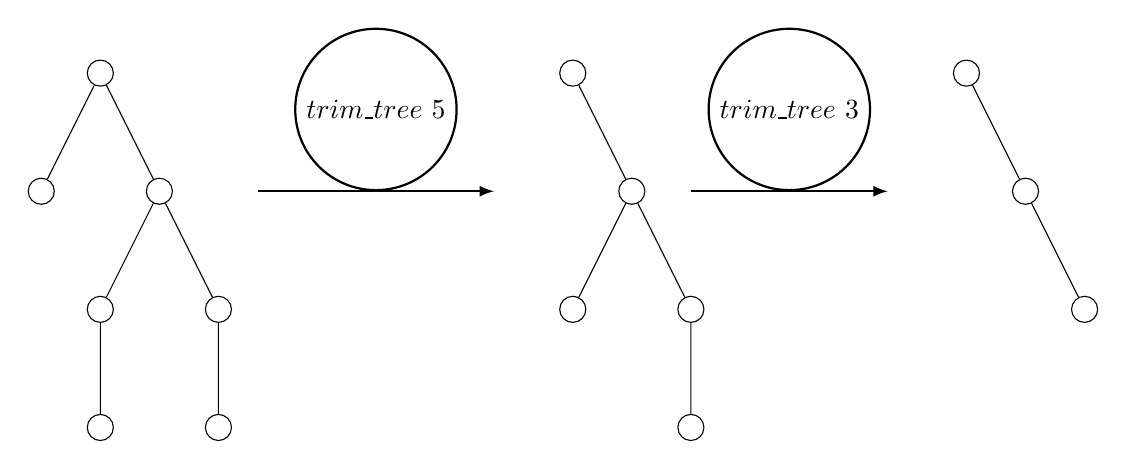
\begin{tikzpicture}
    \begin{scope}[every node/.style={draw,circle}]
        \node {}
        child {node {}}
        child {node {}
            child {node {} child {node {}}}
            child {node {} child {node {}}}};
    \end{scope}

    \draw[-latex,thick] (2.0,-1.5) -- (5,-1.5)
    node[midway,above]{$trim\_tree\ 5$};

    \begin{scope}[xshift=6cm,every node/.style={draw,circle}]
        \node {}
        child[opacity=0] {node {}}
        child {node {}
            child {node {}}
            child {node {} child {node {}}}};
    \end{scope}

    \draw[-latex,thick] (7.5,-1.5) -- (10,-1.5)
    node[midway,above]{$trim\_tree\ 3$};

    \begin{scope}[xshift=11cm,every node/.style={draw,circle}]
        \node {}
        child[opacity=0] {node {}}
        child {node {}
            child[opacity=0] {node {}}
            child {node {}}};
    \end{scope}
    \end{tikzpicture}
\caption{Example of $trim\_tree$}
\label{fig:trim_tree_example}
\end{figure}

\begin{isabellebox}
    \isacommand{fun}\isamarkupfalse%
\ trim{\isacharunderscore}{\kern0pt}tree\ {\isacharcolon}{\kern0pt}{\isacharcolon}{\kern0pt}\ {\isachardoublequoteopen}nat\ {\isasymRightarrow}\ tree\ {\isasymRightarrow}\ nat\ {\isasymtimes}\ tree{\isachardoublequoteclose}\ \isakeyword{where}\isanewline
\ \ {\isachardoublequoteopen}trim{\isacharunderscore}{\kern0pt}tree\ {\isadigit{0}}\ t\ {\isacharequal}{\kern0pt}\ {\isacharparenleft}{\kern0pt}{\isadigit{0}}{\isacharcomma}{\kern0pt}\ t{\isacharparenright}{\kern0pt}{\isachardoublequoteclose}\isanewline
{\isacharbar}{\kern0pt}\ {\isachardoublequoteopen}trim{\isacharunderscore}{\kern0pt}tree\ {\isacharparenleft}{\kern0pt}Suc\ {\isadigit{0}}{\isacharparenright}{\kern0pt}\ t\ {\isacharequal}{\kern0pt}\ {\isacharparenleft}{\kern0pt}{\isadigit{0}}{\isacharcomma}{\kern0pt}\ Node\ {\isacharbrackleft}{\kern0pt}{\isacharbrackright}{\kern0pt}{\isacharparenright}{\kern0pt}{\isachardoublequoteclose}\isanewline
{\isacharbar}{\kern0pt}\ {\isachardoublequoteopen}trim{\isacharunderscore}{\kern0pt}tree\ {\isacharparenleft}{\kern0pt}Suc\ n{\isacharparenright}{\kern0pt}\ {\isacharparenleft}{\kern0pt}Node\ {\isacharbrackleft}{\kern0pt}{\isacharbrackright}{\kern0pt}{\isacharparenright}{\kern0pt}\ {\isacharequal}{\kern0pt}\ {\isacharparenleft}{\kern0pt}n{\isacharcomma}{\kern0pt}\ Node\ {\isacharbrackleft}{\kern0pt}{\isacharbrackright}{\kern0pt}{\isacharparenright}{\kern0pt}{\isachardoublequoteclose}\isanewline
{\isacharbar}{\kern0pt}\ {\isachardoublequoteopen}trim{\isacharunderscore}{\kern0pt}tree\ n\ {\isacharparenleft}{\kern0pt}Node\ {\isacharparenleft}{\kern0pt}t{\isacharhash}{\kern0pt}ts{\isacharparenright}{\kern0pt}{\isacharparenright}{\kern0pt}\ {\isacharequal}{\kern0pt}\isanewline
\ \ {\isacharparenleft}{\kern0pt}case\ trim{\isacharunderscore}{\kern0pt}tree\ n\ {\isacharparenleft}{\kern0pt}Node\ ts{\isacharparenright}{\kern0pt}\ of\isanewline
\ \ \ \ {\isacharparenleft}{\kern0pt}{\isadigit{0}}{\isacharcomma}{\kern0pt}\ t{\isacharprime}{\kern0pt}{\isacharparenright}{\kern0pt}\ {\isasymRightarrow}\ {\isacharparenleft}{\kern0pt}{\isadigit{0}}{\isacharcomma}{\kern0pt}\ t{\isacharprime}{\kern0pt}{\isacharparenright}{\kern0pt}\ {\isacharbar}{\kern0pt}\isanewline
\ \ \ \ {\isacharparenleft}{\kern0pt}n{\isadigit{1}}{\isacharcomma}{\kern0pt}\ Node\ ts{\isacharprime}{\kern0pt}{\isacharparenright}{\kern0pt}\ {\isasymRightarrow}\isanewline
\ \ \ \ \ \ let\ {\isacharparenleft}{\kern0pt}n{\isadigit{2}}{\isacharcomma}{\kern0pt}\ t{\isacharprime}{\kern0pt}{\isacharparenright}{\kern0pt}\ {\isacharequal}{\kern0pt}\ trim{\isacharunderscore}{\kern0pt}tree\ n{\isadigit{1}}\ t\isanewline
\ \ \ \ \ \ in\ {\isacharparenleft}{\kern0pt}n{\isadigit{2}}{\isacharcomma}{\kern0pt}\ Node\ {\isacharparenleft}{\kern0pt}t{\isacharprime}{\kern0pt}{\isacharhash}{\kern0pt}ts{\isacharprime}{\kern0pt}{\isacharparenright}{\kern0pt}{\isacharparenright}{\kern0pt}{\isacharparenright}{\kern0pt}{\isachardoublequoteclose}
\end{isabellebox}

With the help of this a function $fill\_tree$ is defined, $fill\_tree\ n\ t$ produces a list of trees with a total number of $n$ nodes.
Each tree in the list will be $t$ except the first one which might be trimmed to a suitable size in order for the total number of nodes to be $n$.

\begin{isabellebox}
    \isacommand{fun}\isamarkupfalse%
\ fill{\isacharunderscore}{\kern0pt}tree\ {\isacharcolon}{\kern0pt}{\isacharcolon}{\kern0pt}\ {\isachardoublequoteopen}nat\ {\isasymRightarrow}\ tree\ {\isasymRightarrow}\ tree\ list{\isachardoublequoteclose}\ \isakeyword{where}\isanewline
\ \ {\isachardoublequoteopen}fill{\isacharunderscore}{\kern0pt}tree\ {\isadigit{0}}\ {\isacharunderscore}{\kern0pt}\ {\isacharequal}{\kern0pt}\ {\isacharbrackleft}{\kern0pt}{\isacharbrackright}{\kern0pt}{\isachardoublequoteclose}\isanewline
{\isacharbar}{\kern0pt}\ {\isachardoublequoteopen}fill{\isacharunderscore}{\kern0pt}tree\ n\ t\ {\isacharequal}{\kern0pt}\isanewline
\ \ \ \ {\isacharparenleft}{\kern0pt}let\ {\isacharparenleft}{\kern0pt}n{\isacharprime}{\kern0pt}{\isacharcomma}{\kern0pt}\ t{\isacharprime}{\kern0pt}{\isacharparenright}{\kern0pt}\ {\isacharequal}{\kern0pt}\ trim{\isacharunderscore}{\kern0pt}tree\ n\ t\isanewline
\ \ \ \ in\ fill{\isacharunderscore}{\kern0pt}tree\ n{\isacharprime}{\kern0pt}\ t{\isacharprime}{\kern0pt}\ {\isacharat}{\kern0pt}\ {\isacharbrackleft}{\kern0pt}t{\isacharprime}{\kern0pt}{\isacharbrackright}{\kern0pt}{\isacharparenright}{\kern0pt}{\isachardoublequoteclose}
\end{isabellebox}

Now we define the successor function which produces, given a tree, the next smallest canonical tree.
Generating the next smallest tree follows these 4 steps:

\begin{enumerate}
    \item Remove all direct subtrees of the root node which are singleton trees.
    \item Find the first node $v$ (in preorder) which has a singleton tree as the first subtree. Let the subtree of $v$ be $T_v$.
    \item Remove the first singleton subtree of $T_v$ which results in a tree $T_v'$.
    \item Let $p$ be the parent of $v$. Fill the subtree list of $p$ with $T_v'$ until the entire tree consists of $n$ nodes again.
\end{enumerate}

See Figure \ref{fig:next_tree} for examples of how the function operates.

\begin{figure}[htpb]
\centering
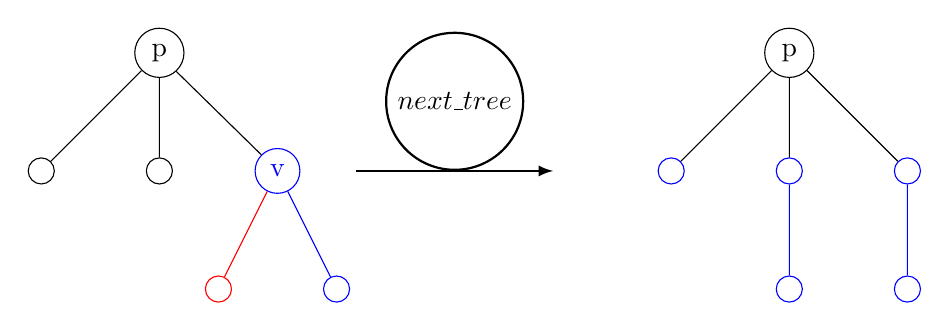
\begin{tikzpicture}
    \begin{scope}[every node/.style={draw,circle}]
        \node {p}
            child {node {}}
            child {node {}}
            child {node[color=blue] (v) {v}
                child[color=red] {node (v1) {}}
                child[color=blue] {node (v2) {}}};
    \end{scope}
    % \node[fit=(v) (v1) (v2), draw] {}

    \draw[-latex,thick] (2.5,-1.5) -- (5,-1.5)
    node[midway,above]{$next\_tree$};

    \begin{scope}[xshift=8cm,every node/.style={draw,circle}]
        \node {p}
            child {node[color=blue] {}}
            child {node[color=blue] {} child[color=blue] {node {}}}
            child {node[color=blue] {} child[color=blue] {node {}}};
    \end{scope}
\end{tikzpicture}

\vspace{1cm}
\centering
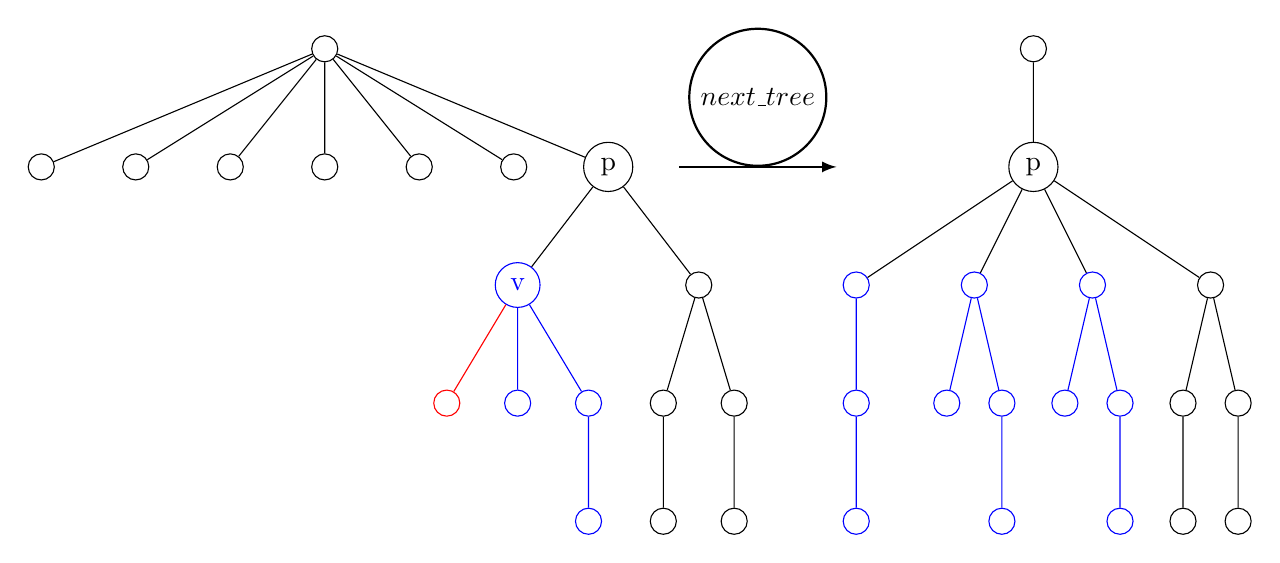
\begin{tikzpicture}
    \begin{scope}[every node/.style={draw,circle},
        level 1/.style={sibling distance=12mm},
        level 2/.style={sibling distance=23mm},
        level 3/.style={sibling distance=9mm}]
        \node {}
            child {node {}}
            child {node {}}
            child {node {}}
            child {node {}}
            child {node {}}
            child {node {}}
            child {node {p}
                child {node[color=blue] {v}
                    child[color=red] {node {}}
                    child[color=blue] {node {}}
                    child[color=blue] {node {} child {node {}}}
                }
                child {node {}
                    child {node {} child {node {}}}
                    child {node {} child {node {}}}
                }
            };
    \end{scope}
    % \node[fit=(v) (v1) (v2), draw] {}

    \draw[-latex,thick] (4.5,-1.5) -- (6.5,-1.5)
    node[midway,above]{$next\_tree$};

    \begin{scope}[xshift=9cm,every node/.style={draw,circle},
        level 1/.style={sibling distance=12mm},
        level 2/.style={sibling distance=15mm},
        level 3/.style={sibling distance=7mm}]
        \node {}
            child {node {p}
                child {node[color=blue] {} child[color=blue] {node {} child {node {}}}}
                child {node[color=blue] {}
                    child[color=blue] {node {}}
                    child[color=blue] {node {} child {node {}}}
                }
                child {node[color=blue] {}
                    child[color=blue] {node {}}
                    child[color=blue] {node {} child {node {}}}
                }
                child {node {}
                    child {node {} child {node {}}}
                    child {node {} child {node {}}}
                }
            };
    \end{scope}
\end{tikzpicture}
\caption{Example of $next\_tree$}
\label{fig:next_tree}
\end{figure}

This function can be directly defined recursively on the tree datatype.

\begin{isabellebox}
    \isacommand{fun}\isamarkupfalse%
    \ next{\isacharunderscore}{\kern0pt}tree{\isacharunderscore}{\kern0pt}aux\ {\isacharcolon}{\kern0pt}{\isacharcolon}{\kern0pt}\ {\isachardoublequoteopen}nat\ {\isasymRightarrow}\ tree\ {\isasymRightarrow}\ tree\ option{\isachardoublequoteclose}\ \isakeyword{where}\isanewline
    \ \ {\isachardoublequoteopen}next{\isacharunderscore}{\kern0pt}tree{\isacharunderscore}{\kern0pt}aux\ n\ {\isacharparenleft}{\kern0pt}Node\ {\isacharbrackleft}{\kern0pt}{\isacharbrackright}{\kern0pt}{\isacharparenright}{\kern0pt}\ {\isacharequal}{\kern0pt}\ None{\isachardoublequoteclose}\isanewline
    {\isacharbar}{\kern0pt}\ {\isachardoublequoteopen}next{\isacharunderscore}{\kern0pt}tree{\isacharunderscore}{\kern0pt}aux\ n\ {\isacharparenleft}{\kern0pt}Node\ {\isacharparenleft}{\kern0pt}Node\ {\isacharbrackleft}{\kern0pt}{\isacharbrackright}{\kern0pt}\ {\isacharhash}{\kern0pt}\ ts{\isacharparenright}{\kern0pt}{\isacharparenright}{\kern0pt}\ {\isacharequal}{\kern0pt}\isanewline
    \ \ \ \ \ \ next{\isacharunderscore}{\kern0pt}tree{\isacharunderscore}{\kern0pt}aux\ {\isacharparenleft}{\kern0pt}Suc\ n{\isacharparenright}{\kern0pt}\ {\isacharparenleft}{\kern0pt}Node\ ts{\isacharparenright}{\kern0pt}{\isachardoublequoteclose}\isanewline
    {\isacharbar}{\kern0pt}\ {\isachardoublequoteopen}next{\isacharunderscore}{\kern0pt}tree{\isacharunderscore}{\kern0pt}aux\ n\ {\isacharparenleft}{\kern0pt}Node\ {\isacharparenleft}{\kern0pt}Node\ {\isacharparenleft}{\kern0pt}Node\ {\isacharbrackleft}{\kern0pt}{\isacharbrackright}{\kern0pt}\ {\isacharhash}{\kern0pt}\ rs{\isacharparenright}{\kern0pt}\ {\isacharhash}{\kern0pt}\ ts{\isacharparenright}{\kern0pt}{\isacharparenright}{\kern0pt}\ {\isacharequal}{\kern0pt}\isanewline
    \ \ \ \ \ \ Some\ {\isacharparenleft}{\kern0pt}Node\ {\isacharparenleft}{\kern0pt}fill{\isacharunderscore}{\kern0pt}tree\ {\isacharparenleft}{\kern0pt}Suc\ n{\isacharparenright}{\kern0pt}\ {\isacharparenleft}{\kern0pt}Node\ rs{\isacharparenright}{\kern0pt}\ {\isacharat}{\kern0pt}\ {\isacharparenleft}{\kern0pt}Node\ rs{\isacharparenright}{\kern0pt}\ {\isacharhash}{\kern0pt}\ ts{\isacharparenright}{\kern0pt}{\isacharparenright}{\kern0pt}{\isachardoublequoteclose}\isanewline
    {\isacharbar}{\kern0pt}\ {\isachardoublequoteopen}next{\isacharunderscore}{\kern0pt}tree{\isacharunderscore}{\kern0pt}aux\ n\ {\isacharparenleft}{\kern0pt}Node\ {\isacharparenleft}{\kern0pt}t\ {\isacharhash}{\kern0pt}\ ts{\isacharparenright}{\kern0pt}{\isacharparenright}{\kern0pt}\ {\isacharequal}{\kern0pt}\isanewline
    \ \ \ \ \ \ Some\ {\isacharparenleft}{\kern0pt}Node\ {\isacharparenleft}{\kern0pt}the\ {\isacharparenleft}{\kern0pt}next{\isacharunderscore}{\kern0pt}tree{\isacharunderscore}{\kern0pt}aux\ n\ t{\isacharparenright}{\kern0pt}\ {\isacharhash}{\kern0pt}\ ts{\isacharparenright}{\kern0pt}{\isacharparenright}{\kern0pt}{\isachardoublequoteclose}\isanewline
    \isanewline
    \isacommand{fun}\isamarkupfalse%
    \ next{\isacharunderscore}{\kern0pt}tree\ {\isacharcolon}{\kern0pt}{\isacharcolon}{\kern0pt}\ {\isachardoublequoteopen}tree\ {\isasymRightarrow}\ tree\ option{\isachardoublequoteclose}\ \isakeyword{where}\isanewline
    \ \ {\isachardoublequoteopen}next{\isacharunderscore}{\kern0pt}tree\ t\ {\isacharequal}{\kern0pt}\ next{\isacharunderscore}{\kern0pt}tree{\isacharunderscore}{\kern0pt}aux\ {\isadigit{0}}\ t{\isachardoublequoteclose}
\end{isabellebox}

None will be returned if the argument is already the smallest tree and thus there is no next smaller tree.

To now enumerate all rooted trees with $n$ nodes,
one starts with the greatest tree on $n$ nodes and repeatedly calls $next\_tree$ until the smallest tree is reached.

\begin{isabellebox}
    \isacommand{fun}\isamarkupfalse%
    \ greatest{\isacharunderscore}{\kern0pt}tree\ {\isacharcolon}{\kern0pt}{\isacharcolon}{\kern0pt}\ {\isachardoublequoteopen}nat\ {\isasymRightarrow}\ tree{\isachardoublequoteclose}\ \isakeyword{where}\isanewline
    \ \ {\isachardoublequoteopen}greatest{\isacharunderscore}{\kern0pt}tree\ {\isacharparenleft}{\kern0pt}Suc\ {\isadigit{0}}{\isacharparenright}{\kern0pt}\ {\isacharequal}{\kern0pt}\ Node\ {\isacharbrackleft}{\kern0pt}{\isacharbrackright}{\kern0pt}{\isachardoublequoteclose}\isanewline
    {\isacharbar}{\kern0pt}\ {\isachardoublequoteopen}greatest{\isacharunderscore}{\kern0pt}tree\ {\isacharparenleft}{\kern0pt}Suc\ n{\isacharparenright}{\kern0pt}\ {\isacharequal}{\kern0pt}\ Node\ {\isacharbrackleft}{\kern0pt}greatest{\isacharunderscore}{\kern0pt}tree\ n{\isacharbrackright}{\kern0pt}{\isachardoublequoteclose}\isanewline
    \isanewline
    \isacommand{function}\isamarkupfalse%
    \ n{\isacharunderscore}{\kern0pt}tree{\isacharunderscore}{\kern0pt}enum{\isacharunderscore}{\kern0pt}aux\ {\isacharcolon}{\kern0pt}{\isacharcolon}{\kern0pt}\ {\isachardoublequoteopen}tree\ {\isasymRightarrow}\ tree\ list{\isachardoublequoteclose}\ \isakeyword{where}\isanewline
    \ \ {\isachardoublequoteopen}n{\isacharunderscore}{\kern0pt}tree{\isacharunderscore}{\kern0pt}enum{\isacharunderscore}{\kern0pt}aux\ t\ {\isacharequal}{\kern0pt}\isanewline
    \ \ {\isacharparenleft}{\kern0pt}case\ next{\isacharunderscore}{\kern0pt}tree\ t\ of\ None\ {\isasymRightarrow}\ {\isacharbrackleft}{\kern0pt}t{\isacharbrackright}{\kern0pt}\ {\isacharbar}{\kern0pt}\ Some\ t{\isacharprime}{\kern0pt}\ {\isasymRightarrow}\ t\ {\isacharhash}{\kern0pt}\ n{\isacharunderscore}{\kern0pt}tree{\isacharunderscore}{\kern0pt}enum{\isacharunderscore}{\kern0pt}aux\ t{\isacharprime}{\kern0pt}{\isacharparenright}{\kern0pt}{\isachardoublequoteclose}\isanewline
    \isacommand{by}\isamarkupfalse%
    \ pat{\isacharunderscore}{\kern0pt}completeness\ auto%
    \isanewline\isanewline
    \isacommand{fun}\isamarkupfalse%
    \ n{\isacharunderscore}{\kern0pt}tree{\isacharunderscore}{\kern0pt}enum\ {\isacharcolon}{\kern0pt}{\isacharcolon}{\kern0pt}\ {\isachardoublequoteopen}nat\ {\isasymRightarrow}\ tree\ list{\isachardoublequoteclose}\ \isakeyword{where}\isanewline
    \ \ {\isachardoublequoteopen}n{\isacharunderscore}{\kern0pt}tree{\isacharunderscore}{\kern0pt}enum\ {\isadigit{0}}\ {\isacharequal}{\kern0pt}\ {\isacharbrackleft}{\kern0pt}{\isacharbrackright}{\kern0pt}{\isachardoublequoteclose}\isanewline
    {\isacharbar}{\kern0pt}\ {\isachardoublequoteopen}n{\isacharunderscore}{\kern0pt}tree{\isacharunderscore}{\kern0pt}enum\ n\ {\isacharequal}{\kern0pt}\ n{\isacharunderscore}{\kern0pt}tree{\isacharunderscore}{\kern0pt}enum{\isacharunderscore}{\kern0pt}aux\ {\isacharparenleft}{\kern0pt}greatest{\isacharunderscore}{\kern0pt}tree\ n{\isacharparenright}{\kern0pt}{\isachardoublequoteclose}
\end{isabellebox}

To prove termination of the enumeration we show that the output of $next\_tree$ (if it is not $None$) is strictly smaller than its input and that there are only finitely many rooted trees with $n$ nodes.

\section{Proof of correctness}

\subsection{Totality}

Instead of working with canonical rooted trees, we work with an alternative (equivalent) definition of regularity.
A rooted ordered tree is regular iff the subtrees are ordered with respect to the linear order previously defined and all subtrees are regular themselves.

\begin{isabellebox}
    \isacommand{fun}\isamarkupfalse%
    \ regular\ {\isacharcolon}{\kern0pt}{\isacharcolon}{\kern0pt}\ {\isachardoublequoteopen}tree\ {\isasymRightarrow}\ bool{\isachardoublequoteclose}\ \isakeyword{where}\isanewline
    \ \ {\isachardoublequoteopen}regular\ {\isacharparenleft}{\kern0pt}Node\ ts{\isacharparenright}{\kern0pt}\ {\isasymlongleftrightarrow}\ sorted\ ts\ {\isasymand}\ {\isacharparenleft}{\kern0pt}{\isasymforall}t{\isasymin}set\ ts{\isachardot}{\kern0pt}\ regular\ t{\isacharparenright}{\kern0pt}{\isachardoublequoteclose}
\end{isabellebox}

To prove correctness we first show that the algorithm enumerates all regular ordered rooted trees and then that the set of regular ordered rooted trees is equivalent to the set of rooted trees modulo isomorphism.

By simple induction all defined functions can be shown to preserve regularity. In addition to that, $next\_tree$ preserves the size of the tree, again by induction and simple auxiliary lemmas on the size of the output of the defined function.
Since $greatest\_tree\ n$ is regular and of size $n$, the algorithm produces only regular trees of size $n$.
Due to the strict monotonicity of $next\_tree$ proven earlier it immediately follows that no tree is generated twice.
In addition, we prove that there is a unique minimal tree of size $n$, namely the tree consisting of a root node and $n-1$ singleton subtrees.
The enumeration stops only if this minimal tree is reached.
What is left to prove is that the algorithm does not skip any regular rooted tree.
For this some auxiliary lemmas are needed.
First, observe that due to the order in which $trim\_tree$ removes nodes, $trim\_tree\ n\ t$ is the greatest tree with at most $n$ nodes that is smaller or equal to $t$.
This also means that a tree which has as subtrees the list of trees generated by $fill\_tree\ n\ t$ is the greatest tree of size $n + 1$ (observe the additional root node) where every subtree is smaller or equal to $t$.
Now to get an intuition of why $next\_tree$ generates the next smallest tree consider counting down numbers as an analogy.
When counting down from $14200$ one tries to decrease the rightmost digit that can be decreased, i.e. the 2.
Then set the digits to the right of the decreased number to their maximum resulting in $14199$.

Since subtrees are compared in reverse order, the leftmost subtree that can be decreased (i.e. is not a singleton) will be decreased by removing its leftmost leaf.
Then using $fill\_tree$ the subtree left to the decreased tree is maximized.
This argument can be made formal by induction on the $next\_tree$ and with some technicalities we omit here.
Thus, we have proven that all regular trees of size $n$ are enumerated by the algorithm.

\begin{isabellebox}
    \isacommand{fun}\isamarkupfalse%
    \ tree{\isacharunderscore}{\kern0pt}size\ {\isacharcolon}{\kern0pt}{\isacharcolon}{\kern0pt}\ {\isachardoublequoteopen}tree\ {\isasymRightarrow}\ nat{\isachardoublequoteclose}\ \isakeyword{where}\isanewline
    \ \ {\isachardoublequoteopen}tree{\isacharunderscore}{\kern0pt}size\ {\isacharparenleft}{\kern0pt}Node\ ts{\isacharparenright}{\kern0pt}\ {\isacharequal}{\kern0pt}\ Suc\ {\isacharparenleft}{\kern0pt}{\isasymSum}t{\isasymleftarrow}ts{\isachardot}{\kern0pt}\ tree{\isacharunderscore}{\kern0pt}size\ t{\isacharparenright}{\kern0pt}{\isachardoublequoteclose}\isanewline
    \isanewline
    \isacommand{definition}\isamarkupfalse%
    \ regular{\isacharunderscore}{\kern0pt}n{\isacharunderscore}{\kern0pt}trees\ {\isacharcolon}{\kern0pt}{\isacharcolon}{\kern0pt}\ {\isachardoublequoteopen}nat\ {\isasymRightarrow}\ tree\ set{\isachardoublequoteclose}\ \isakeyword{where}\isanewline
    \ \ {\isachardoublequoteopen}regular{\isacharunderscore}{\kern0pt}n{\isacharunderscore}{\kern0pt}trees\ n\ {\isacharequal}{\kern0pt}\ {\isacharbraceleft}{\kern0pt}t{\isachardot}{\kern0pt}\ tree{\isacharunderscore}{\kern0pt}size\ t\ {\isacharequal}{\kern0pt}\ n\ {\isasymand}\ regular\ t{\isacharbraceright}{\kern0pt}{\isachardoublequoteclose}%
    \isanewline\isanewline
    \isacommand{theorem}\isamarkupfalse%
    \ {\isachardoublequoteopen}set\ {\isacharparenleft}{\kern0pt}n{\isacharunderscore}{\kern0pt}tree{\isacharunderscore}{\kern0pt}enum\ n{\isacharparenright}{\kern0pt}\ {\isacharequal}{\kern0pt}\ regular{\isacharunderscore}{\kern0pt}n{\isacharunderscore}{\kern0pt}trees\ n{\isachardoublequoteclose}
\end{isabellebox}

\subsection{Distinctness modulo Isomorphism}

In order for the algorithm to meet its specification we need to show that the regular ordered rooted trees are equivalent to all rooted trees.
We define a function to map an ordered unlabeled rooted tree to a rooted labeled tree in graph form.
This is done via two additional intermediate steps which simplify the proofs.
First we define ordered rooted labeled trees which are like ordered rooted trees except that each node has a label associated with it.
A function is defined to label the nodes of an unlabeled tree.
This can be done arbitrarily as long as the nodes have different labels since any labeling will produce an isomorphic tree.
Next we define unordered labeled trees where the subtrees of a node are represented as a finite set instead of an ordered list.
As the last step one can transform an unordered labeled tree $t$ into its graph representation simply by the graph $G = (V,E)$ where $V$ is the set of nodes in $t$ and $E$ contains an edge for every node to the roots of its subtrees.
Let $t$ be an ordered unlabeled rooted tree, then $G_t$ denotes the graph representation of $t$.
It can be shown that $G_t$ is indeed a tree, i.e. connected and acyclic.

We now want to show for every tree graph $T$ there exists exactly one $t$ such that $T$ and $G_t$ are isomorphic.
Let $r$ be the root of $T$.
Moreover, let $C$ be the set of connected components of $T - \{r\}$ (the tree without its root). 
Then one can generate unordered unlabeled trees for each connected component recursively by taking the unique vertex in it that is connected to $r$ as its root.
The sorted list of these trees will be the subtrees of $t$.
This construction results in a regular tree $t$ such that $G_t$ is isomorphic to $T$.
Denote this tree by $t(T)$.

The remaining step to show uniqueness is to show that $G_{t_1}$ and $G_{t_2}$ are not isomorphic for two distinct regular trees $t_1$ and $t_2$, or equivalently that $t_1 = t_2$ is implied by $G_{t_1}$ and $G_{t_2}$ being isomorphic.
\begin{isabellebox}
    \isacommand{lemma}\isamarkupfalse%
    {\kern0pt}\ {\isachardoublequoteopen}regular\ t{\isadigit{1}}\ {\isasymLongrightarrow}\ regular\ t{\isadigit{2}}\ {\isasymLongrightarrow}\ G\isactrlsub {t{\isadigit{1}}}\ {\isasymsimeq}\isactrlsub r\ G\isactrlsub {t{\isadigit{2}}}\ {\isasymLongrightarrow}\ t{\isadigit{1}}\ {\isacharequal}{\kern0pt}\ t{\isadigit{2}}{\isachardoublequoteclose}
\end{isabellebox}
One can prove that $t(G_t) = t$ for all regular trees t.
Also, since the construction of $t(T)$ does not depend on the labels of the nodes, but only on the structure of the tree, we have $t(G_{t_1}) = t(G_{t_2})$ since $G_{t_1}$ and $G_{t_2}$ are isomorphic.
This means
\[
    t1 = t(G_{t_1}) = t(G_{t_2}) = t2
\]
which finishes the proof.

This concludes the entire proof and shows that the described algorithm generates each tree exactly once modulo isomorphic, that is it generates all unlabeled rooted trees.

\begin{isabellebox}
    \isacommand{theorem}\isamarkupfalse%
    \ {\isachardoublequoteopen}G\ {\isasymin}\ n{\isacharunderscore}{\kern0pt}rtree{\isacharunderscore}{\kern0pt}graphs\ n\isanewline
    \ \ \ \ {\isasymLongrightarrow}\ {\isasymexists}{\isacharbang}{\kern0pt}G{\isacharprime}{\kern0pt}\ {\isasymin}\ set\ {\isacharparenleft}{\kern0pt}n{\isacharunderscore}{\kern0pt}rtree{\isacharunderscore}{\kern0pt}graph{\isacharunderscore}{\kern0pt}enum\ n{\isacharparenright}{\kern0pt}{\isachardot}{\kern0pt}\ G{\isacharprime}{\kern0pt}\ {\isasymsimeq}\isactrlsub r\ G{\isachardoublequoteclose}
\end{isabellebox}
